\cleardoublepage


\chapter{Pfadplanung}\label{ch:pfadplanung}

Pfadplanungsalgorithmen werden häufig in der Robotik und der Automatisierungstechnik eingesetzt, um Pfade für Roboter oder Maschinen zu beschreiben, die sich innerhalb eines bestimmten Arbeitsbereichs bewegen.
Dabei werden eine Reihe an Konfigurationen zu berechnet, die den Weg von einer bestimmten Transformation in eine andere beschreiben.
Eine einzelne Konfiguration ist im Falle des UR5 ein Tupel mit sechs Winkeln, das die Ausrichtung der sechs Gelenke des Roboters angibt.

In dieser Arbeit wird hierzu insbesondere zwischen dem direkten und kürzesten Weg unterschieden.
Der kürzeste Weg ist die im kartesischen Raum direkte Verbindung zwischen einem Start- und einem Zielpunkt (Abschnitt~\ref{sec:kurzesterweg}), wobei die Rotation ebenfalls linear angepasst wird.
Im Gegensatz dazu wird beim direkten Weg eine Zielkonfiguration des Roboters mit konstanter Geschwindigkeit der Gelenke angefahren.
Beschränkungen, wie Kollisionen mit der Umgebung oder mit sich selbst, können die Berechnung der Pfade allerdings erschweren.

In diesem Kapitel sollen die Grundlagen der Pfadplanung, sowie die Algorithmen zur Implementierung der obigen Planungsoptionen näher vorgestellt werden.


\section{Konfigurationsraum}\label{sec:konfigurationsraum}

Der Konfigurationsraum $\mathit{C}$ stellt die Grundlage für die Algorithmen in der Pfadplanung dar und beschreibt alle möglichen Konfigurationen, die der Roboter einnehmen kann.
Eine Konfiguration des UR5 ist dabei wie in Gleichung~\ref{eq:config-1} definiert, wobei die Winkelwerte $\theta_i$ durch ihre Maximal- und Minimalwerte des Datenblatts~\cite{universalrobotsUR5TechnicalSpecifications} von $\pm 360^{\circ}$ beschränkt sind.
Gleichsam existieren Konfigurationen innerhalb dieser Menge $\mathit{O}\in\mathit{C}$, die Kollisionen beschreiben.
Darunter zählen Konfigurationen, bei denen sich der Roboter selbst im Weg steht, sowie welche, bei denen der Untergrund oder statische Hindernisse eine erfolgreiche Ausführung der Bewegung verhindern.
Der für die Pfadplanung relevante Bereich ist demzufolge der in Gleichung~\ref{eq:config-2} beschriebene Menge $\mathit{C}_{free}$, der freie Konfigurationsraum, dessen Konfigurationen den Bereich beschreiben, durch den Roboter sich bewegen kann~\cite[83f]{sicilianoRobotics2009}.

\begin{equation}
    \mathit{C} = \left\{ \left( \theta_1,\dots,\theta_6 \right) \in \theta_1\times\dots\times\theta_6 \mid \theta_i \in \left[ -2\pi, 2\pi \right]\right\}
    \label{eq:config-1}
\end{equation}
\begin{equation}
    \mathit{C}_{free} = \mathit{C}\backslash\mathit{O}
    \label{eq:config-2}
\end{equation}

Je nach Algorithmus muss der Konfigurationsraum allerdings nicht im vorhinein berechnet werden, insbesondere wenn der Konfigurationsraum sehr groß ist oder dynamisch Hindernisse erkannt werden sollen.
Um Kollisionen einfach und schnell berechnen zu können wurde in dieser Arbeit ein auf zehn Grad genauer Kollisionsraum vollständig berechnet und in einer Bibliothek abgespeichert.
Um Kollisionen abzufragen, wird die Suchkonfiguration dafür immer auf den nächstmöglichen vorberechneten Wert auf- oder abgerundet.
Es könnte allerdings schneller und genauer sein, die Kollisionen stattdessen während der Laufzeit mit einer externen Bibliothek zu berechnen.


\section{Pfad des kürzesten Weges}\label{sec:kurzesterweg}

Der kürzeste Weg bezeichnet die Bewegung des Roboters, der die geringste Translationsbewegung des Endeffektors zur Folge hat, und entspricht einer Geraden zwischen Start- und Zielpunkt (siehe Abbildung~\ref{fig:pth1}).
Um dies zu berechnen, wird die Strecke zunächst in mehrere Zwischenstufen zwischen zwei oder mehr Transformationspunkten $T_1$ und $T_2$ unterteilt.
Jeder Schritt kann dabei mithilfe des Faktors $t \in \left[0,1\right]$ beschrieben werden (Gleichung~\ref{eq:shortest-path-1}).
Zwischen zwei Rotationsmatrizen $R_1$ und $R_2$  wird in der Regel der sogenannte Slerp verwendet  (Gleichung~\ref{eq:shortest-path-2}), der jedoch erst in Quaternionen ($Q_1$ und $Q_2$) umgerechnet werden muss.
Zu beachten sind zudem die Rechenregeln der Quaternionen, die hier nicht näher erklärt werden.

\begin{equation}
    P_{t} = P_0 + \left( P_1 - P_0 \right) \cdot t
    \label{eq:shortest-path-1}
\end{equation}
\begin{equation}
    Q_{t} = Q_1 \cdot \left( Q_1^{-1} \cdot Q_2 \right)^t
    \label{eq:shortest-path-2}
\end{equation}

Die resultierende Liste von Endeffektor-Transformationen muss im Anschluss mithilfe der inversen Kinematik aus Abschnitt~\ref{ch:inverse-kinematik} in den Konfigurationsraum des Roboters übertragen werden.
Der UR5 hat, wie in Abschnitt~\ref{sec:geometrische-losung} berechnet, für jede Zwischentransformation oftmals bis zu acht, oder in einer Singularität sogar unendlich viele Stellungen für die Gelenke.
Dabei werden Konfigurationen, bei denen eine Kollision besteht, entfernt und Singularitäten durch Addition eines kleinen Werts $\epsilon$ umgangen.

Anschließend wird ein gerichteter Graph erstellt, dessen Knoten die Konfigurationen der Zwischentransformationen darstellen, die Kanten die Übergänge zwischen diesen Konfigurationen beschreiben und deren Kantenlängen die Summe der Winkeldifferenzen aller Konfigurationen benachbarter Zeitschritte ausweisen.
Nachdem der Graph erstellt wurde, müssen alle Knoten, die nicht vom Startknoten erreichbar sind, mithilfe einer Breitensuche entfernt werden.
Danach kann zum Beispiel mit Dijkstra der kürzeste Weg im Graph beschrieben werden, der in diesem Fall genau den Weg darstellt, bei dem sich die Gelenke am wenigsten bewegen müssen.

\begin{figure}[h]
    \centering
    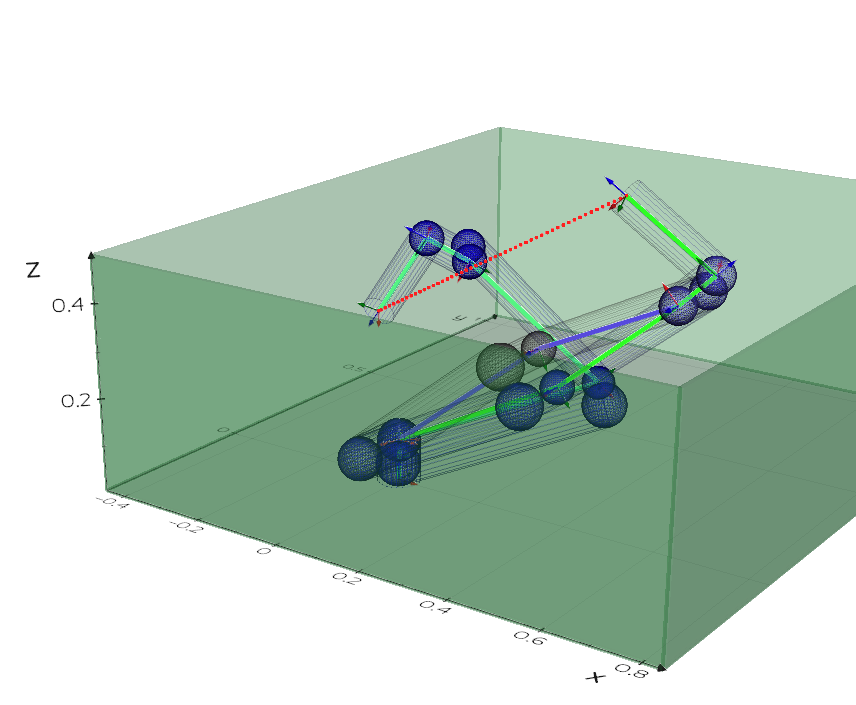
\includegraphics[width = .8\textwidth]{Bilder/shortestpath}
    \caption{Beispiel eines kürzesten Pfades zwischen zwei Endeffektor-Trans\-for\-ma\-tio\-nen mit Zwischenpunkten}\label{fig:pth1}
\end{figure}


\section{Pfad der direkten Bewegung}\label{sec:direkterweg}

Um von einer Start- in eine Zielkonfiguration zu fahren, können die Zielwinkel auch alle direkt linear angefahren werden.
Dafür werden die Zwischenpositionen für jedes Gelenk mit Startwinkel $\theta_{i_0}$ und Zielwinkel $\theta_{i_1}$ mithilfe des Faktors $t \in \left[0,1\right]$ berechnet (Gleichung~\ref{eq:dir-1}).
Da die Winkelbeschränkungen des UR5 bei $\pm 360^\circ$ liegen, existieren für jeden Winkel $\theta_{i_1}$ bis zu zwei Alternativwinkel.
Die Menge der Zielwinkel erweitert sich dabei wie in Gleichung~\ref{eq:dir-2}.

\begin{equation}
    \theta_{i_t} = \theta_{i_0} + t \cdot \left(  \theta_{i_1} -  \theta_{i_0} \right)  \label{eq:dir-1}
\end{equation}
\begin{equation}
    \Theta_i = \left\{ \theta_{i_1} + x \lvert x \in \left\{ -360, 0, 360 \right\} \wedge x \in BOUNDS  \right\}
    \label{eq:dir-2}
\end{equation}



Mit den sechs Freiheitsgraden des UR5 ergeben sich damit in der Regel $2^{6}=64$ Pfade zur Zielkonfiguration.
Werden allerdings für eine Zieltransformation acht mögliche Zielkonfigurationen betrachtet, steigt dieser Wert auf $8\cdot 64=512$ Pfade.
In der Implementierung kann dann der kürzeste der kollisionsfreien Pfade gewählt und ausgeführt werden.

Die resultierende Bewegung des Endeffektors ist dabei bei dieser Methode nicht linear und ergibt nach Auswahl des kürzesten Pfads ergibt der Algorithmus meist einen flachen Bogen (Abbildung~\ref{fig:pth2}).

\begin{figure}[h]
    \centering
    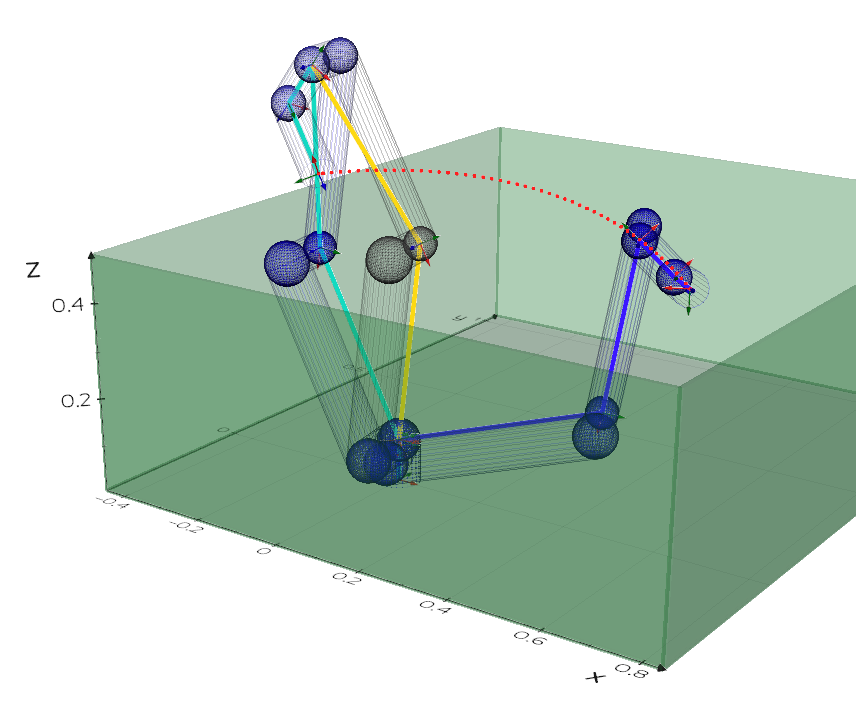
\includegraphics[width = .8\textwidth]{Bilder/directpath}
    \caption{Beispiel eines direkten Pfades zwischen zwei Endeffektor-Trans\-for\-ma\-tio\-nen mit Zwischenpunkten}\label{fig:pth2}
\end{figure}


\section{Implementierung}

Im Code stehen verschiedene Beispiele zur Ausführung zur Verfügung.
Nach Installation der \enquote{requirements.txt} kann die Datei \enquote{main.py} gestartet werden, um eine zufallsbasierte Demo der beiden obigen Algorithmen durchzuführen.
Es wird zunächst eine zufällige Start- und Zielkonfiguration gewählt und dann eine Suche nach einem kürzesten Pfad durchgeführt.
Bei einem Fehlschlag wird auf den direkten Weg als alternative Methode zurückgegriffen.
Die besten Ergebnisse können im Anschluss in der Simulation betrachtet werden.
Dieses Vorgehen wiederholt sich für andere zufällige Parameter weiter.
Alternativ können die folgenden Beispiele und Funktionen aber auch direkt ausgeführt werden:

\begin{itemize}
    \item \enquote{calculate\_obstacle\_space()} zur Neuberechnung aller möglichen Selbstkollisionen (lange Rechenzeit)
    \item \enquote{inverse\_kinematics\_example()} Anzeige aller acht Konfigurationen für eine gegebene Endeffektor-Transformation
    \item \enquote{direct\_path\_example()} Anzeige der kürzesten fünf direkten Wege für die Aufgabe
    \item \enquote{shortest\_path\_example()} Anzeige des kürzesten Wegs für die Aufgabe, mit Fallback auf vorherige Methode.
\end{itemize}

%\subsection{Zellendekomposition}\label{subsec:zellendekomposition}
%?? Quelle
%
%In der Zellendekomposition wird der freie Konfigurationsraum $C_{free}$ in kleinere Felder, sog.\ Zellen unterteilt.
%Zwei Konfigurationen liegen genau dann in der gleichen Zelle, falls ein Übergang zwischen den beiden Zuständen kollisionsfrei möglich ist und zwei benachbarte Zellen müssen über einen einfachen Pfad miteinander kollisionsfrei verbunden sein.
%Dies setzt konvexe Zellen voraus, bei denen jeder Punkt innerhalb der Zelle jeden anderen erreichen kann.
%Auf Basis dieser Gruppierungen kann dann ein Konnektivitätsgraph oder eine Roadmap erstellt werden.
%Als Datenstruktur kann ein KD-Tree verwendet werden, der ein Konfigurationsraum als Baum so abbildet, dass Abstände und benachbarte Zellen zügig berechnet werden können.
%Im zweidimensionalen Raum werden hierfür die Positionen und Dimensionen von Quadraten sowie dessen Nachbarn gespeichert.
%
%Diese direkte Berechnung der Zellenstruktur ist im sechsdimensionalen Fall des UR5 allerdings nichttrival und aufwändig.
%Aus diesem Grund und für die schnellere Berechnung wird deshalb oftmals eine approximierte Lösung aus einem Sampling-Verfahren bevorzugt.

%\subsection{Sampling-Verfahren}
%?? Quelle
%
%In Sampling-basierten Verfahren wird das Gruppieren aller Konfigurationen in konkave Zellen übersprungen und stattdessen nur einzelne, benötigte Konfigurationen auf Kollision geprüft.
%Das bedeutet, dass nicht die beste Lösung aller möglichen Lösungen ermittelt wird, sondern nur die beste aller bereits ermittelten Lösungen.
%Der Algorithmus kann dementsprechend bereits nach dem Finden der ersten Lösung terminieren.
%Bedingung dafür ist allerdings eine Möglichkeit, eine Konfiguration schnell auf Kollisionsfreiheit zu überprüfen zu können.
%Insofern der Konfigurationsraum vollständig bekannt ist oder schon zuvor berechnet wurde, kann alternativ auch ein Lookup-Table verwendet werden.
%
%Im Folgenden wird zwischen Single- und Multi-Query-Verfahren unterschieden:

%\subsubsection{Single-Query Verfahren}
%
%Bei Single-Query-Verfahren wird für jede Abfrage ein neuer Weg gesucht, bei Multi-Query-Verfahren werden vergangene Anfragen als Hilfestellung für neue Anfragen genutzt und so eine Roadmap erzeugt.
%Üblicherweise wird beim Single-Query-Verfahren mit Startkonfiguration $q_a$ und Zielkonfiguration $q_b$ wie folgt vorgegangen:
%\begin{enumerate}
%    \item Initalisierung eines Graphens $G(V, E)$ mit Knoten mit $V=\left\{ q_a, q_b \right\}$ und $E=\left\{  \right\}$
%    \item Auswahl eines Expansionsknotens aus $V$ mit einem gewählten Algorithmus
%    \item Berechnung eines neuen Knotens und einer Kante mit einem gewählten Algorithmus (inklusive Kollisionsüberprüfung)
%    \item Erweiterung des Graphens mit zuvor gefundenem Knoten und neuer Kante (falls möglich).
%    \item Prüfe auf Lösung in G (Verbindung von Start und Zielknoten) oder wiederhole ab 2.
%\end{enumerate}
%
%Zudem kann der Algorithmus auf zwei oder mehr Suchbäume ausgeweitet werden, die sich nach einiger Zeit in der Mitte treffen.
%Dazu wird dann in den Schritten 2\-4 der verwendete Baum zufällig ausgewählt.
%
%Der \ac{rrt} ist ein häufig verwendeter Suchbaum in diesem Kontext.
%Hier wird zunächst wie in 3.\ eine neue Konfiguration zufällig gewählt und ab dem nächsten Knoten im Graphen eine Schrittweite in Richtung dieser Konfiguration gegangen.
%Um einen Bias gegenüber der Zielkonfiguration zu erzeugen, kann zudem mit einer gewissen Wahrscheinlichkeit der zufällig gewählte Knoten mit dem tatsächlichen Zielknoten ersetzt werden.
%Bei RRT$^*$ wird bei der Erweiterung zusätzlich auf andere Verbindungen des Graphens zum neu berechneten Knoten geprüft, was die Länge der kürzesten Verbindung zwischen Start und Ziel noch einmal minimiert.
%Die kürzeste Verbindung kann beispielsweise mithilfe von A$^*$ oder Dijkstra ermittelt werden.
%
%\subsubsection{Multi-Query}
%Bei Multi-Query Verfahren können bereits berechnete Kanten des aufgebauten Graphens wiederverwendet werden.
%Im Probabilistic-Roadmap-Algorithmus werden in einem ersten Schritt n zufällige Knotenpunkte erzeugt und dann mit ihren nächsten Nachbarn verbunden, insofern keine Kollision vorliegt.
%Im Anschluss werden Start- und Zielknoten ergänzt und ebenfalls Nachbarn als Kanten im Graphen hinzugefügt.
%Am Ende kann dann wieder mithilfe von A$^*$ oder Dijkstra ein kürzester Weg ermittelt werden.
%
%
%??
%
%%Single-Query
%%Unidirektional vs.\ Bidirektional
%%RRT
%%biased / unbiased to exploration
%%Q-space muss nicht vollständig bekannt sein
%%RRT*
%%Multi-Query
%%Probabilistic Roadmaps
%Potentialfeldmethode / Gradientenverfahren
%Genetische Algorithmen
%
%


%\section{Praxisbezug}\label{sec:praxisbezug}
%Kinematisch (Winkelbegrenzung)
%Dynamisch (Geschwindigkeit)
%Einbezug der Constraints in den Algorithmen
%Praxis: OMPL (MoveIt+ ROS / Copelliasim Plugin)


%
%Pfadplanungsalgorithmen können dazu beitragen, komplexe Pfade in einem Konfigurationsraum zu beschreiben.
%ROS (Robot Operating System) und CopelliaSim bieten bereits Frameworks, die dieses Problem lösen.
%
%Da in dieser Arbeit der Schwerpunkt auf der Selbstkollision bei der Pfadplanung liegen soll und die inverse Kinematik nahezu ohne Singularitäten direkt berechnet werden kann, kann ein deutlich vereinfachter Algorithmus verwendet werden.
%Das setzt allerdings voraus, dass der Kollisionsraum schon zu Beginn der Berechnung vollständig bekannt ist.
%Aus diesen Gründen wurde in der Implementierung eine Bibliothek für das Überprüfen von Selbstkollisionen angelegt, in der alle möglichen Transformationen des UR5 auf fünf Grad genau abgespeichert sind.
%
%Im implementierten Algorithmus kann zunächst für jede Zwischentransformation, die in Abschnitt~\ref{sec:kurzesterweg} beschrieben wurde, mithilfe der inversen Kinematik aus Abschnitt~\ref{ch:inverse-kinematik} eine Liste möglicher Zwischenkonfigurationen erstellt werden.
%Dabei werden Konfigurationen, bei denen eine Kollision besteht, entfernt und Singularitäten durch das Addieren eines kleinen Werts $\epsilon$ umgangen.
%
%Anschließend wird ein Graph erstellt, dessen Knoten die Konfigurationen der Zwischentransformationen darstellen, die Kanten die Übergänge zwischen diesen Konfigurationen beschreiben und deren Kantenlängen die Summe der Winkeldifferenzen aller Konfigurationen benachbarter Zeitschritte ausweisen.
%Nachdem der Graph erstellt wurde, müssen alle Knoten, die nicht vom Startknoten erreichbar sind, mithilfe einer Breitensuche entfernt werden.
%Danach kann zum Beispiel mit Dijkstra der kürzeste Weg im Graph beschrieben werden, der in diesem Fall genau den Weg darstellt, bei dem sich die Gelenke am wenigsten bewegen müssen.
%
